

\chapter{Examining the impact of dynamism on pattern rewriting in static and dynamic languages}
\label{chap:dynamism-pattern-rewriting}

% Hook
% Argument
% Link

\section{Quantifying the performance impact of dynamism in language runtimes}

% Hook
% Argument
% Link

% TODO: Could unmerge C++ and Python?
\subsection{Dynamism in C++}

% Hook
% Argument
% Link

\subsection{Cost of dynamic dispatch}

%% Introduce vtables etc.
% Hook
% Argument
% Link

%% Perf table/graph

%% Empirical performance of vtables vs static calls
% Hook
% Argument
% Link

\subsection{Dynamism hiding ahead-of-time optimisations}

%% Introduce common optimisations
% Hook
% Argument
% Link

%% How can we construct an experiment to show these being hidden?
% Hook
% Argument
% Link

%% Perf table/graph

%% Discussion of results
% Hook
% Argument
% Link

\subsection{Runtime type information}

%% Introduce RTTI machinery
% Hook
% Argument
% Link

%% How can we construct an experiment to show these?
% Hook
% Argument
% Link

%% Perf table/graph

%% Discussion of results
% Hook
% Argument
% Link



\subsection{Dynamism in Python}

% Hook
% Argument
% Link

\subsection{Specialised and unspecialised instructions}

% Hook
% Argument
% Link

%% Perf table/graph

%% Discussion of results
% Hook
% Argument
% Link

\subsection{Runtime type information}
% Hook
% Argument
% Link

%% Perf table/graph

%% Discussion of results
% Hook
% Argument
% Link






\section{Dynamism in xDSL}

% Hook
% Argument
% Link

\subsection{Operation trait checks}

% Hook
Having specialised xDSL's \mintinline{python}{has_trait} method to the most minimal implementation which expresses the desired functionality, we can draw comparisons between equivalent algorithms which predominantly measure the effect of the language runtime.
% Argument
Both implementations (Listing \ref{listing:ubenchmark-trait-checks-both}) share the same underlying algorithm: iteration over an operations traits, checking against each one. However, the mechanism used for this algorithm differs significantly between xDSL and MLIR.
By leveraging Python's dynamic nature, xDSL can invoke the \mintinline{python}{isinstance} function to check each trait. In contrast, MLIR uses template metaprogramming instead of the class hierarchy to define traits. This depends on \mintinline{c++}{TypeID}\footnote{\url{https://mlir.llvm.org/doxygen/TypeID_8h_source.html}}, a custom data structure to encode dynamic \ac{rtti} in C++.
% TODO: Does this need more detail?
Whilst this implementation incurs complexity (\autoref{fig:ubenchmark-hastrait-dynamism}), it remains performant, as the \mintinline{c++}{TypeID} data structure is constructed to remedy many of the issues of native C++ \ac{rtti}.
% Link
However, this dynamism impacts performance beyond just the runtime of the individual function, as it presents an optimisation boundary -- precluding other optimisations which could be applied if the result could be inferred at compile time. % TODO: This really needs to be substantiated somehow, but perhaps not here?

\begin{figure}[H]
    \centering
    \begin{subfigure}[b]{\textwidth}
        
\includegraphics[width=\textwidth]{images/impact_dynamism/hastrait_xdsl_viztracer_optimised.png}
        \caption{\texttt{viztracer} trace of xDSL's optimised \mintinline{python}{has_trait} implementation.}
        \label{fig:ubenchmark-hastrait-xdsl-viztracer-optimised}
    \end{subfigure}
    \begin{subfigure}[b]{\textwidth}
        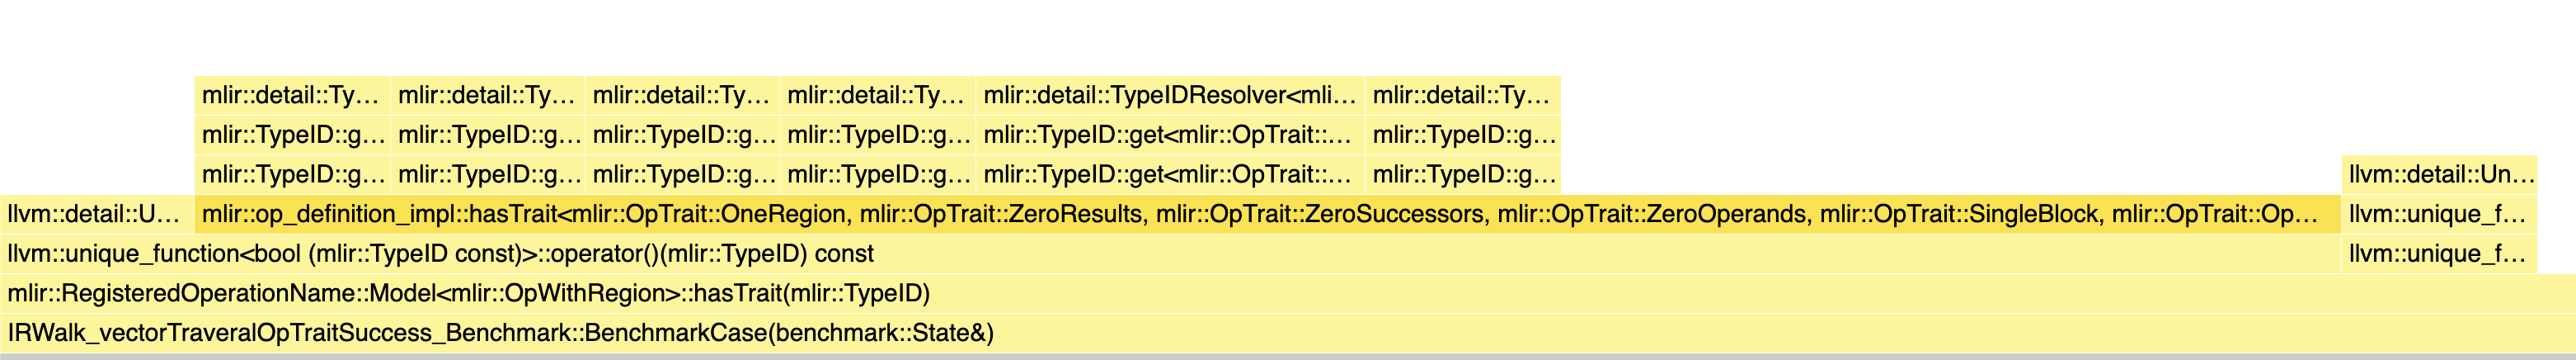
\includegraphics[width=\textwidth]{images/impact_dynamism/hastrait_mlir_samply.png}
        \caption{\texttt{samply} trace of MLIR's \mintinline{c++}{has_trait} method.}
        \label{fig:ubenchmark-hastrait-mlir-samply}
    \end{subfigure}
    \caption{MLIR's dynamic trait checking using C++ RTTI is more complex than xDSL's Python implementation using \mintinline{python}{isinstance}.}
    \label{fig:ubenchmark-hastrait-dynamism}
\end{figure}


\subsection{Constant folding}

% Hook
% Argument
% Link

% Hook
% Argument
% Link

% Hook
% Argument
% Link


\section{Summary}

% Hook
% Argument
% Link

% Hook
% Argument
% Link
